\begin{figure}[H]
\scalebox{0.5}{%
    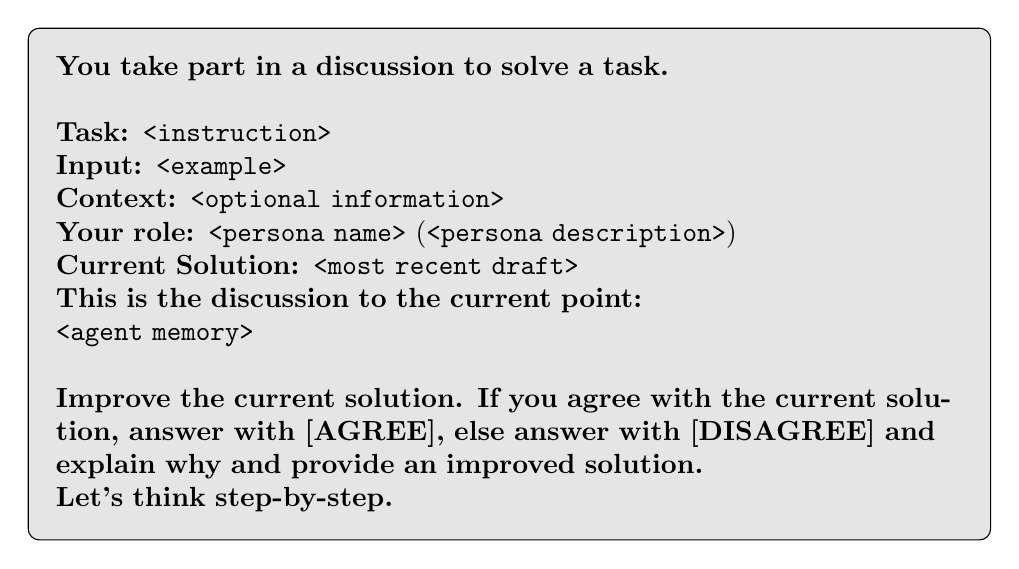
\begin{tikzpicture}
    \node [draw, rectangle, rounded corners, fill=gray!20, text width=0.95\textwidth, inner sep=10pt] (block) {
        \begin{minipage}{\textwidth}
        \textbf{You take part in a discussion to solve a task.} \\

        \textbf{Task:} \texttt{<instruction>} \\
        \textbf{Input:} \texttt{<example>} \\
        \textbf{Context:} \texttt{<optional information>} \\
        \textbf{Your role:} \texttt{<persona name>} (\texttt{<persona description>}) \\
        \textbf{Current Solution:} \texttt{<most recent draft>}

        \textbf{This is the discussion to the current point:} \\
        \texttt{<agent memory>} \\

        \textbf{Improve the current solution. If you agree with the current solution, answer with [AGREE], else answer with [DISAGREE] and explain why and provide an improved solution.} \\
        \textbf{Let's think step-by-step.}
        \end{minipage}
    };
    \end{tikzpicture}
}
\caption{Prompt to an agent that contributes to the discussion. If this is the first message of the discussion, we write "Nobody proposed a solution yet. Please provide the first one." instead of the most recent draft and agent memory.}
\end{figure}
